\subsection{Target Density}\label{sec:analysis.target_density}

We need to know the target density to calculate the differential cross-section. The procedure for determining the density of $\ell$H$_2$ target in \abbr{CLAS} has already been established in ~\cite{clas.target.density}. In the \desg{g12} experiment, the target temperature and pressure was measured periodically during each run. Each run contained at least 3 measurements of the pressure and temperature. The formula for calculating the target density is;
% ~\cite{clas.target.density}
\begin{align}
\rho = a_1T^2 + a_2P +a_3 \label{eq:target_density} \ ,
\end{align} 
where $T$ and $P$ represent the temperature and pressure respectively and $a_1$, $a_2$, $a_3$ are constants given in Tab.~\ref{tab:targetdensity} taken from ~\cite{mccarty}. Fig.~\ref{fig:target_density} shows the average target density, $\bar \rho$, for each run along with the $\sqrt{\sigma^2}$.
\begin{table}[h!]
\begin{minipage}{\textwidth}
\begin{center}
\begin{singlespacing}

\caption[Target Density Constants]{\label{tab:targetdensity}Constants used in target density measurements \vspace{0.75mm}}

\begin{tabular}{c|c}

%\hline \hline
%
%operation & \multicolumn{3}{c}{Generation} \\
%charge & I & II & III \\

\hline
Parameter & Value \\
\hline

$a_{1}$ & $-2.89 \cdot 10^{-5} \frac{g}{cm^3K^2}$  \\
$a_{2}$ & $1.0 \cdot 10^{-7} \frac{g}{cm^3mbar}$  \\
$a_{3}$ & $8.249 \cdot 10^{-2} \frac{g}{cm^3}$  \\
\hline \hline
\end{tabular}

\end{singlespacing}
\end{center}
\end{minipage}
\end{table}
\vspace{20pt}
The average density, for each run, was calculated as;
\begin{align}
\bar \rho_{run} = \frac{1}{N}\sum_i^N \rho_i \ ,
\end{align} 
while the variance $\sigma^2$ is calculated, for each run, as;
\begin{align}
\sigma^2 = \frac{1}{N - 1}\sum_i^N (\rho_i - \bar \rho)^2 \ .
\end{align}
Once the target density was calculated for each run, the average target density for all \desg{g12} runs was calculated using;
\begin{align}
\bar \rho_{tot} = \frac{1}{N_{run}}\sum_i^{N_{run}} \bar \rho_{run} = 0.0711398 \pm 1.74 \cdot10^{-5}\ ,
\end{align} 
while the variance $\sigma^2$ is calculated, for all \desg{g12} run, as;
\begin{align}
\sigma_{tot}^2 = \frac{1}{N_{run} -1}\sum_i^{N_{run}} (\bar \rho_{run} - \bar \rho_{tot})^2 = 0.00024 \ .
\end{align}
Since the uncertainty, $\sigma$, in the target density is lower than the uncertainty of the physical in the target materials, the target density uncertainty will not be a factor in the total systematic errors, Sec.\ref{sec:results.systematics}. The target length has an inaccuracy of 40~cm $\pm$ 0.2~cm. This gives a systematic of 0.5\%. 

\begin{figure}[h!]\begin{center}
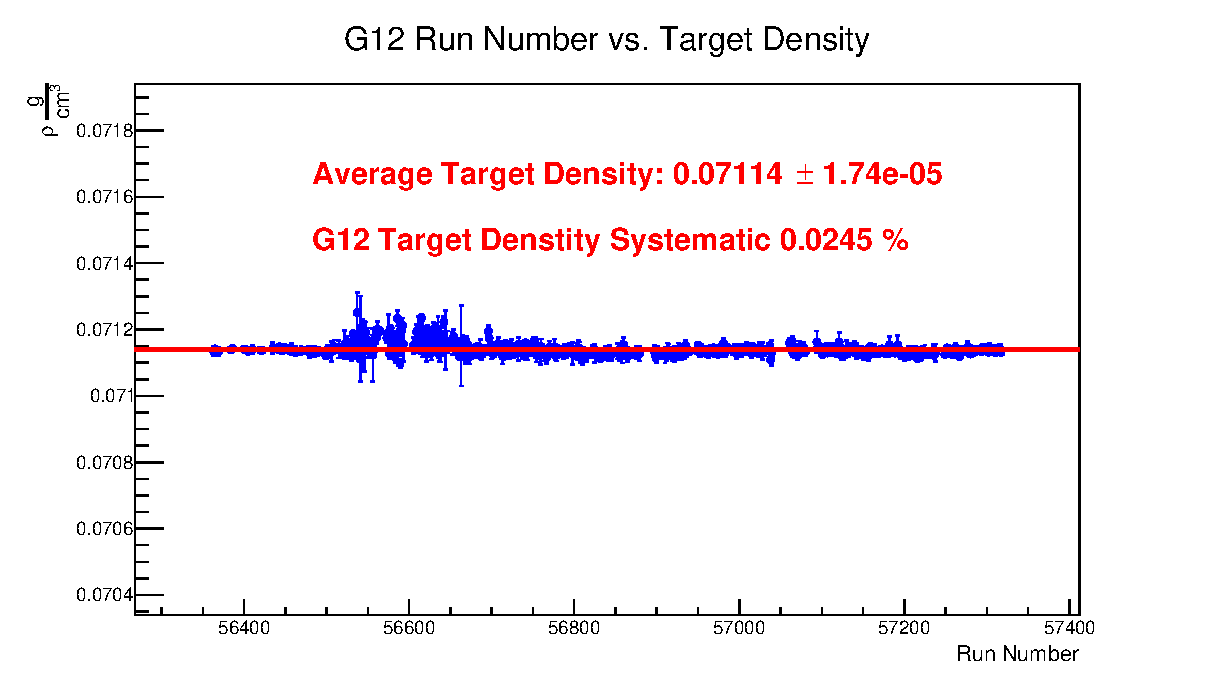
\includegraphics[width=0.9\textwidth]{figures/calib/targ/G12_Target_Density.eps}
\caption[Target density for \desg{g12}]{\label{fig:target_density}Target density for \desg{g12}. Image source:~\cite{clas.thesis.kunkel}}
\end{center}\end{figure}
\FloatBarrier